\documentclass[../../Rapport RayTracer]{subfiles}

\begin{document}


Afin de parser n'importe quel fichier au format pov, la méthode qui a été retenu est celle du pattern State. Ce pattern s'est révélé être le plus adapté pour implémenter un automate à états finis. Voici, ci-dessous, le diagramme de classe de notre pattern state avec les classes d'état qui l'implémentent:

\begin{figure}[h!]
	\adjustbox{center}{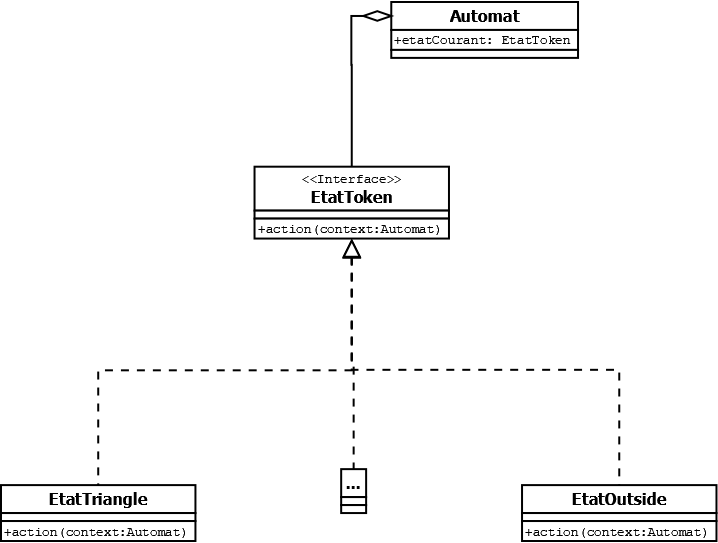
\includegraphics[width=1\textwidth]{diagrammes/pattern_state.png}}
	
	\caption{Diagramme du pattern state appliqué à notre parser}
	\label{diagrammePatternState}
\end{figure}
\FloatBarrier

Ce pattern est composé d'une interface EtatToken qui définit une méthode action qui servira à parser le bon objet. Ensuite, on crée ce que l'on appelle des classes d'état qui implémentent l'interface et donc redéfinissent la méthode action. Ce sont elles qui s'occupent de tout le traitement de la figure. Ces classes correspondent à un seul objet/figure à la fois, à l'exception de la classe EtatSpherePlane dont on parlera plus tard. Cette interface est donc en quelque sorte le modèle d'un état.
On a ensuite notre classe principale, la classe Automat qui possède un attribut de type EtatToken. Le grand avantage de ce pattern se trouve dans cette classe. Au lieu d'avoir chaque état dans la classe Automat, on a un seul état type, celui de l'interface. Dès que l'on se trouve sur une certaine figure on change l'état courant et on appelle sa méthode action. La méthode action possède en argument le contexte d'exécution de l'automate, c'est important notamment pour récupérer l'instance courante du streamTokenizer et donc sa dernière position dans le fichier. Voici un exemple de fonctionnement d'un appel d'état:

 \lstinputlisting[language=Java]{../../code/exemple_appel_state.java}

Et voici la méthode action de la classe Automat (qui n'a rien à voir avec celle des états):

 \lstinputlisting[language=Java]{../../code/actionMethod.java}
 
Elle nous sert simplement à appeler la méthode action de l'interface.

\end{document}